\documentclass[12pt]{article}
\usepackage[utf8]{inputenc}
\usepackage{geometry}
\geometry{letterpaper, margin=0.25in}
\usepackage{graphicx} 
\usepackage{parskip}
\usepackage{booktabs}
\usepackage{array} 
\usepackage{paralist} 
\usepackage{verbatim}
\usepackage{subfig}
\usepackage{fancyhdr}
\usepackage{sectsty}
\usepackage[shortlabels]{enumitem}

\pagestyle{fancy}
\renewcommand{\headrulewidth}{0pt} 
\lhead{}\chead{}\rhead{}
\lfoot{}\cfoot{\thepage}\rfoot{}

%%% ToC (table of contents) APPEARANCE
\usepackage[nottoc,notlof,notlot]{tocbibind} 
\usepackage[titles,subfigure]{tocloft}
\renewcommand{\cftsecfont}{\rmfamily\mdseries\upshape}
\renewcommand{\cftsecpagefont}{\rmfamily\mdseries\upshape} %

\usepackage{amsmath}
\usepackage{amssymb}
\usepackage{mathtools}
\usepackage{empheq}
\usepackage{xcolor}
\usepackage{bbm}
\usepackage{tikz}
\usepackage{pgfplots}
\usepackage{tikz-cd}
\pgfplotsset{compat=1.18}

\newcommand{\ans}[1]{\boxed{\text{#1}}}
\newcommand{\vecs}[1]{\langle #1\rangle}
\renewcommand{\hat}[1]{\widehat{#1}}

\renewcommand{\P}{\mathbb{P}}
\newcommand{\R}{\mathbb{R}}
\newcommand{\E}{\mathbb{E}}
\newcommand{\Z}{\mathbb{Z}}
\newcommand{\N}{\mathbb{N}}
\newcommand{\Q}{\mathbb{Q}}
\newcommand{\C}{\mathbb{C}}

\newcommand{\ind}{\mathbbm{1}}
\newcommand{\qed}{\quad \blacksquare}

\newcommand{\brak}[1]{\left\langle #1 \right\rangle}
\newcommand{\bra}[1]{\left\langle #1 \right\vert}
\newcommand{\ket}[1]{\left\vert #1 \right\rangle}

\newcommand{\abs}[1]{\left\vert #1 \right\vert}
\newcommand{\mfX}{\mathfrak{X}}
\newcommand{\ep}{\varepsilon}

\newcommand{\Ec}{\mathcal{E}}
\newcommand{\A}{\mathcal{A}}
\newcommand{\F}{\mathcal{F}}
\newcommand{\Cc}{\mathcal{C}}
\newcommand{\B}{\mathcal{B}}
\newcommand{\M}{\mathcal{M}}
\newcommand{\X}{\chi}
\renewcommand{\L}{\mathcal{L}}

\newcommand{\sub}{\subseteq}
\newcommand{\st}{\text{ s.t. }}
\newcommand{\card}{\text{card }}
\renewcommand{\div}{\vspace*{10pt}\hrule\vspace*{10pt}}
\newcommand{\surj}{\twoheadrightarrow}
\newcommand{\inj}{\hookrightarrow}
\newcommand{\biject}{\hookrightarrow \hspace{-8pt} \rightarrow}
\renewcommand{\bar}[1]{\overline{#1}}
\newcommand{\overcirc}[1]{\overset{\circ}{#1}}
\newcommand{\diam}{\text{diam }}

\renewcommand{\Re}{\text{Re}\,}
\renewcommand{\Im}{\text{Im}\,}
\newcommand{\sign}{\text{sign}\,}

\newcommand*{\tbf}[1]{\ifmmode\mathbf{#1}\else\textbf{#1}\fi}

\usepackage{tcolorbox}
\tcbuselibrary{breakable, skins}
\tcbset{enhanced}
\newenvironment*{tbox}[2][gray]{
    \begin{tcolorbox}[
        parbox=false,
        colback=#1!5!white,
        colframe=#1!75!black,
        breakable,
        title={#2}
    ]}
    {\end{tcolorbox}}

\newenvironment*{exercise}[1][red]{
    \begin{tcolorbox}[
        parbox=false,
        colback=#1!5!white,
        colframe=#1!75!black,
        breakable
    ]}
    {\end{tcolorbox}}

\newenvironment*{proof}[1][blue]{
\begin{tcolorbox}[
    parbox=false,
    colback=#1!5!white,
    colframe=#1!75!black,
    breakable
]}
{\end{tcolorbox}}

\DeclareMathOperator{\Prob}{\mathbb{P}}
\DeclareMathOperator{\Exp}{\mathbb{E}}
\DeclareMathOperator{\Var}{\mathbb{V}}
\DeclareMathOperator*{\argmin}{\arg\min}
\DeclareMathOperator{\SSS}{\mathcal{S}}
\newcommand{\bs}{\boldsymbol}
\newcommand{\be}{\begin{enumerate}}
\newcommand{\ee}{\end{enumerate}}
\newcommand{\teq}{\triangleq}

\title{APMA 1740 Homework 1}
\author{Milan Capoor}
\date{31 Jan 2025}

\begin{document}
\maketitle

\begin{enumerate}[1.]

	\item[] \hspace{-3ex} {\bf For 1740 and 2610:}

	\item {\bf Convex functions of one variable.} Loosely speaking, a convex function is bowl shaped. Formally speaking, a convex function satisfies \[ f(\lambda x + (1-\lambda)y) \leq \lambda f(x)+(1-\lambda)f(y) \] for every distinct pair $x\neq y$ and every $0\leq \lambda\leq 1$, which says that the graph of the function lies below the chord connecting any two points on the graph.\footnote{If you fix the points $x$ and $y$ and vary $\lambda$ from $0$ to $1$, then $f(\lambda x + (1-\lambda)y)$ traces out the values of the function between $x$ and $y$. Similarly, $\lambda f(x)+(1-\lambda)f(y)$ traces out the values of the straight line between $f(x)$ and $f(y)$. So $f(\lambda x + (1-\lambda)y) \leq \lambda f(x)+(1-\lambda)f(y)$ is a way to say that the graph of a function lies below the chord connecting any two points on the graph.}

	      If a function is everywhere twice differentiable, then it is convex if and only if (iff) its second derivative is nonnegative: $f''(x)\geq 0$ for all $x$. A function $g$ is concave if $-g$ is convex. (So concave functions are like upside-down bowls.) A function is {\em strictly} convex if

	      \[ f(\lambda x + (1-\lambda)y) < \lambda f(x)+(1-\lambda)f(y) \]
	      for every distinct pair $x\neq y$ and every $0 < \lambda < 1$, and this can be verified by further showing that $f''(x)>0$ everywhere, except perhaps at isolated points.

	      \begin{center}
		      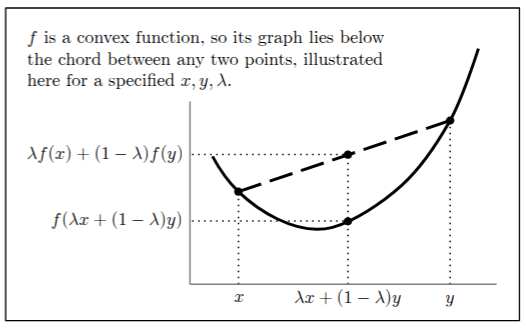
\includegraphics[width=0.5\textwidth]{Images/HW1-convex.png}
	      \end{center}

	      \begin{enumerate}
		      \item Prove that $f(x)=x^2$ is strictly convex. (Hint. Show that $f''(x)> 0$ for all $x$.)
		            \color{blue}
		            \begin{align*}
			            f'(x) = 2x & \implies f''(x) = 2 > 0 \quad \forall x \\
			                       & \implies f \text{ strictly convex.}
		            \end{align*}
		            \color{black}
		      \item Prove that $f(x)=\log x$ is strictly concave for $x > 0$.
		            \color{blue}
		            \begin{align*}
			            g(x) := -\log x & \implies g' = -\frac{1}{x}                           \\
			                            & \implies g'' = \frac{1}{x^2} > 0 \quad \forall x > 0 \\
			                            & \implies g \text{ strictly convex}                   \\
			                            & \implies f \text{ strictly concave.}
		            \end{align*}
		            \color{black}
		      \item Prove that $f(x)=x\log x$ is strictly convex for $x > 0$.
		            \color{blue}
		            \begin{align*}
			            f'(x) = 1 + \log x & \implies f''(x) = \frac{1}{x} > 0 \quad \forall x > 0 \\
			                               & f \text{ strictly convex.}
		            \end{align*}
		            \color{black}
		      \item Prove that $f(x)=ax+b$ is both convex and concave for any choice of $a,b$.

		            \color{blue}
		            \begin{align*}
			            f'(x) = a  & \implies f''(x) = 0 \geq 0 \quad \forall x \\
			                       & \implies f \text{ convex}                  \\
			            g'(x) = -a & \implies f''(x) = 0 \geq 0 \quad \forall x \\
			                       & \implies f \text{ concave}
		            \end{align*}
		            \color{black}
	      \end{enumerate}

	      \pagebreak
	\item {\bf Convex functions of many variables.} More generally, a convex function $f(x)$, where $x=(x_1,\dotsc,x_s)$ is a vector, satisfies the same inequality: \[ f(\lambda x + (1-\lambda)y) \leq \lambda f(x)+(1-\lambda)f(y) \] for every distinct pair $x\neq y$ and every $0\leq \lambda\leq 1$. The intuitions are nearly identical. And $g$ is concave if $-g$ is convex. Verifying that a function of many variables is convex can be a little more tricky, however. One way to do it is to prove that the new function
	      \[ h(\lambda) = f(\lambda x + (1-\lambda) y) \]
	      is convex for $0\leq \lambda \leq 1$ and every fixed (and distinct) choice of $x$ and $y$. This is nice, because $h$ is now a function of one variable, so you might be able to compute the second derivative of $h$ and verify that it is nonnegative: $h''(\lambda)\geq 0$ on $[0,1]$. If you can additionally verify that $h''(\lambda)>0$ on $(0,1)$, then $f$ is strictly convex (just like in problem 2).
	      \begin{enumerate}
		      \item Prove that $f(x)=\sum_{i=1}^s (w_i x_i)^2$ is a convex function, where $w=(w_1,\dotsc,w_s)$ is a fixed vector of real numbers.  (Hint: Show that the function $h(\lambda)=f(\lambda x+(1-\lambda)y)=\sum_{i=1}^s (w_i(\lambda x_i +(1-\lambda) y_i))^2$ is convex for every choice of $x$ and $y$ and for $0\leq\lambda\leq 1$. And show that $h(\lambda)$ is convex by showing that $h''(\lambda)\geq 0$.)

		            \color{blue}
		            \begin{align*}
			            h(\lambda)   & =\sum_{i=1}^s w_i^2 (\lambda x_i +(1-\lambda) y_i)^2               \\
			            h'(\lambda)  & = \sum_{i=1}^s 2w_i^2(\lambda x_i - \lambda y_i + y_i) (x_i - y_i) \\
			            h''(\lambda) & = \sum_{i=1}^s 2w_i^2 x_i(x_i - y_i) - 2w_i y_i(x_i - y_i)         \\
			                         & = \sum_{i=1}^s \underbrace{2w_i^2(x_i - y_i)^2}_{\geq 0}\; \geq 0
		            \end{align*}
		            Hence, $f$ is convex.
		            \color{black}

		      \item Prove that $f(x) = -\sum_{i=1}^s x_i\log x_i$ is a strictly concave function for $x\in(0,\infty)^s$, meaning that each $x_i > 0$.\footnote{By defining $0\log 0=0$, we can extend $f$ to a continuous function on $[0,\infty)^s$, so that it is strictly concave on all of $[0,\infty)^s$. You do not have to prove this.} Note: If $x$ is a pmf, then $f(x)=H(x)$ is the entropy of $x$, so you have just proved that entropy is a strictly concave function.

		            \color{blue}
		            \allowdisplaybreaks
		            \begin{align*}
			            h(\lambda)   & = -\sum_{i=1}^s (\lambda x_i + (1 - \lambda) y_i) \log(\lambda x_i + (1 - \lambda) y_i)                                                                                                            \\
			                         & = -\sum_{i=1}^s \lambda x_i \log(\lambda x_i + (1 - \lambda) y_i) + (1 - \lambda) y_i \log(\lambda x_i + (1 - \lambda) y_i)                                                                        \\
			            h'(\lambda)  & = -\sum_{i=1}^s x_i \log(\lambda x_i + (1 - \lambda) y_i) + \frac{\lambda x_i \cdot (x_i - y_i)}{\lambda x_i + y_i - \lambda y_i}  + \frac{y_i \cdot (x_i - y_i)}{\lambda x_i + y_i - \lambda y_i} \\
			                         & \qquad - y_i \log(\lambda x_i + y_i - \lambda y_i) - \frac{\lambda y_i \cdot (x_i - y_i)}{\lambda x_i + y_i - \lambda y_i}                                                                         \\
			                         & = -\sum_{i=1}^{s} (x_i - y_i) \log(\lambda x_i + y_i - \lambda y_i) + \frac{(x_i - y_i)(\lambda x_i + y_i- \lambda y_i)}{\lambda x_i + y_i - \lambda y_i}                                          \\
			                         & = -\sum_{i=1}^{s} (x_i - y_i) \log(\lambda x_i + y_i - \lambda y_i) + (x_i - y_i)                                                                                                                  \\
			            h''(\lambda) & = -\sum_{i=1}^{s} \frac{(x_i - y_i)^2}{\lambda x_i + (1- \lambda) y_i}
		            \end{align*}

		            Now since $x_i, y_i \in (0, \infty)^s$, $x_i \neq y_i$, and $\lambda \in [0, 1]$, we have that $\frac{(x_i - y_i)^2}{\lambda x_i + (1- \lambda) y_i} > 0$.

		            In particlar, this means that $h''(\lambda) < 0$, so $h$ is stritly concave. Hence, $f$ is strictly concave.
		            \color{black}


		      \item Prove that $f(x) = \sum_{i=1}^s x_i\log (x_i/w_i)$ is a strictly convex function for $x\in(0,\infty)^s$, where $w$ is a fixed vector of positive numbers. (The previous footnote applies here, as well.)
		            Note: If $x$ and $w$ are pmfs, then $f(x)=D(x\|w)$ is called the relative entropy of $w$ with respect to $x$, so you have just proved that relative entropy is a strictly convex function in the first argument.

		            \color{blue}
		            \begin{align*}
			            h(\lambda)   & = \sum_{i=1}^s (\lambda x_i + (1 - \lambda) y_i) \log\left(\frac{\lambda x_i + (1 - \lambda) y_i}{w_i}\right)                                                                     \\
			            h'(\lambda)  & = \sum_{i=1}^{s} (x_i - y_i) \log\left(\frac{\lambda x_i + (1 - \lambda)y_i}{w_i}\right) + \frac{w_i(\lambda x_i + (1 - \lambda y_i))(x_i - y_i)}{\lambda x_i + (1 - \lambda)y_i} \\
			                         & = \sum_{i=1}^{s} (x_i - y_i) \log\left(\frac{\lambda x_i + (1 - \lambda)y_i}{w_i}\right) + w_i(x_i - y_i)                                                                         \\
			            h''(\lambda) & = \sum_{i=1}^{s} \frac{w_i(x_i - y_i)^2}{\lambda x_i + (1 - \lambda)y_i}
		            \end{align*}

		            Again, $x_i, y_i \in (0, \infty)^s$ with $x_i \neq y_i$, $w_i \in (0, \infty)^s$, and $\lambda \in [0, 1]$. Hence, $\frac{w_i(x_i - y_i)^2}{\lambda x_i + (1 - \lambda)y_i} > 0$. So $h''(\lambda) > 0$ and $h$ and $f$ are strictly convex.
		            \color{black}
	      \end{enumerate}


	      \pagebreak
	\item {\bf Jensen's inequality}. Let $f$ be a convex function. Consider the inequality
	      \[ f\bigg(\sum_{i=1}^s p_i x_i\bigg) \leq \sum_{i=1}^s p_i f(x_i)  \quad \quad \text{ for all $x_1,\dotsc,x_s$ and all pmfs $p=p_{1:s}$.} \]
	      \begin{enumerate}
		      \item Prove the inequality for $s=1$. (This is trivial.)

		            \color{blue}
		            We WTS that $f(p x) \leq p f(x)$. But $p = p_1$ is a PMF, so $p = 1 \implies f(x) \leq f(x)$. Trivial.
		            \color{black}

		      \item Prove the inequality for $s=2$. (This is very easy, since $f$ is convex.)

		            \color{blue}
		            WTS $f(p_1x_1 + p_2x_2) \leq p_1f(x_1) + p_2f(x_2)$. But $p_1 + p_2 = 1$, so equivalently,
		            \[f(p_1 x_1 + (1 - p_1)x_2 \leq p_1 f(x_1) + (1 - p_1)f(x_2))\]
		            which is precisely the condition for convexity of $f$.

		            \color{black}

		      \item Prove the inequality for $s=3$. (Hint: Use convexity twice.)

		            \color{blue}
		            Suppose not. Notice $p_1 + p_2 + p_3 = 1$.

		            Assume WLOG $p_2, p_3 \neq 0$ (else we reduce to the $s = 1$ case). Let $y = \frac{p_2 x_2 + p_3 x_3}{p_2 + p_3}$. Then
		            \begin{align*}
			            f(\sum_{i=1}^3 p_i x_i) & = f(p_1 x_1 + (p_2 + p_3) y)                                                                                                            \\
			                                    & = f(p_1 x_1 + (1 - p_1) y)                                                                                                              \\
			                                    & \leq p_1 f(x_1) + (1 - p_1) f(y)                                                                          & (\text{by convexity of } f) \\
			                                    & = p_1 f(x_1) + (p_2 + p_3)\cdot f\left(\frac{p_2}{p_2 + p_3} x_2 + \frac{p_3}{p_2 + p_3} x_3\right)                                     \\
			                                    & = p_1 f(x_1) + (p_2 + p_3)\cdot f\left(\frac{p_2}{p_2 + p_3} x_2 + (1 - \frac{p_2}{p_2 + p_3}) x_3\right)                               \\
			                                    & = p_1 f(x_1) + (p_2 + p_3)\left[\frac{p_2}{p_2 + p_3} f(x_2) + (1 - \frac{p_2}{p_2 + p_3}) f(x_3)\right]  & (\text{by convexity of } f) \\
			                                    & = p_1 f(x_1) + (p_2 + p_3)\left[\frac{p_2}{p_2 + p_3} f(x_2) + \frac{p_3}{p_2 + p_3}f(x_3)\right]                                       \\
			                                    & = p_1 f(x_1) + p_2 f(x_2) + p_3 f(x_3)                                                                                                  \\
			                                    & = \sum_{i=1}^3 p_i f(x_i) \qed
		            \end{align*}
		            \color{black}


		      \item Assume that the inequality is true for $s=m$. Prove that it must therefore also be true when $s=m+1$.

		            (Hint: By taking $m=3$, you can use the previous two parts to prove the $s=m+1=4$ case, and then repeat forever to prove the inequality for any choice of $s$. This method of proof is called {\em induction})

		            \color{blue}
		            Suppose $f$ convex and
		            \[f\left(\sum_{i=1}^m p_i x_i\right) \leq \sum_{i=1}^m p_i f(x_i)\]

		            Notice
		            \begin{align*}
			            f\left(\sum_{i=1}^{m+1} p_i x_i\right) & = f\left(\sum_{i=1}^m p_i x_i + p_{m+1}x_{m+1}\right)                                                               \\
			                                                   & = f\left(p_{m+1}x_{m+1} + (1 - p_{m+1})\sum_{i=1}^m \frac{p_i}{1 - p_{m+1}} x_i\right)                              \\
			                                                   & = p_{m+1} f(x_{m+1})+ (1 - p_{m+1}) f\left(\sum_{i=1}^m \frac{p_i}{1 - p_{m+1}} x_i\right) & (\text{by convexity})  \\
			                                                   & \leq p_{m+1} f(x_{m+1}) + (1 - p_{m+1})\sum_{i=1}^m \frac{p_i}{1 - p_{m+1}} f(x_i)         & (\text{by assumption}) \\
			                                                   & = p_{m+1} f(x_{m+1} ) + \sum_{i=1}^m p_i f(x_i)                                                                     \\
			                                                   & = \sum_{i=1}^{m+1} p_i f(x_i)
		            \end{align*}

		            By induction, the inequality holds for all $s$. $\qed$
		            \color{black}

		      \item Let $X$ be a random variable with a pmf $p=p_{1:s}$. Prove Jensen's inequality: $f(\Exp(X))\leq \Exp(f(X))$.
		            (Really, there's nothing left to do---just apply the definitions of the expressions on the two sides of the inequality.)

		            \color{blue}
		            \begin{align*}
			            f(\E X) & = f\left(\sum_{i=1}^s p_i x_i\right)                              \\
			                    & \leq \sum_{i=1}^s p_i f(x_i)         \qquad \text{(by (d) above)} \\
			                    & = \E f(X) \qed
		            \end{align*}
		            \color{black}
	      \end{enumerate}

	      \pagebreak
	\item {\bf Empirical distributions.} The empirical distribution is random, so it has its own distribution, which is confusing. It gets even more confusing when we sample many empirical distributions, so that we can have empirical distributions of empirical distributions. This problem takes you through some of the details and will hopefully make things clearer. Let $X_{1:n}=(X_1,\dotsc,X_n)$ be an independent and identically distributed (iid) sequence with common pmf $h=h_{1:s}=(h_1,\dotsc,h_s)$. The empirical distribution (or, more accurately, the empirical pmf) of $X_{1:n}$ is the vector $\widehat p=\widehat p_{1:s}$ defined by
	      \[ \widehat p_x = \widehat p_x(X_{1:n}) = \frac{1}{n}\sum_{i=1}^n \ind\{X_i=x\} = \frac{\#\{i:X_i=x\}}{n} . \]
	      The second expression emphasizes that $\widehat p$ depends on the realization of $X_{1:n}$. The third expression illustrates that $\widehat p_x$ is a sum of iid random variables, which is helpful for computing expected values or thinking about the law of large numbers.
	      \begin{enumerate}
		      \item Show that $\widehat p$ is a pmf for every possible sequence $X_{1:n}$.

		            \color{blue}
		            It suffices to show that
		            \begin{enumerate}
			            \item $\sum_x \hat p_x = 1$
			            \item $\hat p_x \geq 0$ for all $x$
		            \end{enumerate}

		            Choose any $X_{1:n}$. Then
		            \begin{align*}
			            \sum_x \hat p_x & = \sum_x \frac{1}{n} \sum_{i=1}^n \ind\{X_i = x\}       \\
			                            & = \frac{1}{n} \sum_{i=1}^n \sum_{x=1}^s \ind\{X_i = x\} \\
			                            & = \frac{1}{n} \sum_{i=1}^n 1                            \\
			                            & = 1
		            \end{align*}

		            Further, by definition of the counting measure, $\#\{i: X_i = x\} \geq 0$ so for $n > 0$,
		            \[\hat p_x = \frac{\#\{i: X_i = x\}}{n} \geq 0\]

		            Hence, $\hat p$ is a pmf for every possible sequence $X_{1:n}$.
		            \color{black}

		      \item Argue that $\widehat p$ is random, so it is a random pmf.

		            \color{blue}
		            $\hat p_x$ is a function of $X_i$ and the constant $n$. Since $X_i$ are random, $\hat p_x$ is random.
		            \color{black}

		      \item Since $\widehat p$ is random, it has an expected value. Compute $\Exp(\widehat p)$ in terms of $s$, $h$, and $n$, where $\Exp$ denotes expected value.\footnote{The expected value of a vector is just the vector of the expected values of the components, so, for instance, $\Exp(\widehat p) = (\Exp(\widehat p_1),\dotsc,\Exp(\widehat p_s))$.}

		            \color{blue}
		            Since $\E(\hat p) = (\E \hat p_1, \E \hat p_2, \dots, \E \hat p_s)$, it suffices to compute $\E [\hat p_x]$ for any $x$:
		            \begin{align*}
			            \E [\hat p_x] & = \E\left[\frac{1}{n} \sum_{i=1}^n \ind\{X_i = x\}\right]                                        \\
			                          & = \frac{1}{n} \sum_{i=1}^n \E[\ind\{X_i = x\}]               & (\text{linearity of expectation}) \\
			                          & = \frac{1}{n} \sum_{i=1}^n [1 \cdot h_x + 0 \cdot (1 - h_x)]                                     \\
			                          & = \frac{1}{n} \sum_{i=1}^n h_x                                                                   \\
			                          & = h_x
		            \end{align*}

		            So $\E[\hat p] = h$.
		            \color{black}

		      \item For $n=s^{100}$ what will $\widehat p$ be very close to with high probability. Why?

		            \color{blue}
		            The formula $\hat p_x = \frac{1}{n }\sum_{i=1}^n \ind\{X_i = x\}$ tell us that $\hat p_x$ is the average of $n$ iid Bernoulli random variables with parameter $h_x$. By the law of large numbers,
		            \[\hat p_x \overset{a.s.}{\longrightarrow} \E[\ind\{X_i = x\}] = 1 \cdot h_x + 0 \cdot (1 - h_x) = h_x\]

		            In particular, this means that for $n = s^{100}$, $\hat p \approx h$.
		            \color{black}


		      \item Since $\widehat p$ is random, it also has a pmf, say $r$, given by
		            \[ r_q = \Prob(\widehat p = q) \]
		            for any pmf $q$.
		            Give an exact expression for $r_q$ in terms of $s$, $h$, $q$, and $n$. Make sure to indicate in your expression those $q$ for which $r_q=0$. For $s=3$, $h=(1/3,1/3,1/3)$, $q=(0.5,0.3,0.2)$ and $n=10$, compute the value of $r_q$.

		            \color{blue}
		            \[r_q = \P(\hat p = q) = \binom{n}{n q_1, \dots, n q_s} \prod_{i=1}^s h_i^{n q_i}\]

		            Hence, for $s=3$, $h=(1/3,1/3,1/3)$, $q=(0.5,0.3,0.2)$ and $n=10$,
		            \begin{align*}
			            r_q & = \binom{10}{5, 3, 2} \left(\frac{1}{3}\right)^5 \left(\frac{1}{3}\right)^3 \left(\frac{1}{3}\right)^2 \\
			                & =  \frac{10!}{5!\, 3!\, 2!} \left(\frac{1}{3}\right)^{10}                                              \\
			                & = 2520 \cdot \frac{1}{59049}                                                                           \\
			                & = \boxed{\frac{280}{6561}}
		            \end{align*}
		            \color{black}
		      \item {\color{blue} (Do not submit)} For the case $s=3$ and $h=(1/3,1/3,1/3)$ and arbitrary $n$, write a function that generates a random observation from the pmf $r$. Except for very small $n$, you can't actually construct the pmf $r$ because there are too many possible candidate pmfs $q$. But you can still sample from it by simply creating a random $\widehat p$.\footnote{For this $s$ and $h$, you can get a random $X_{1:n}$ in Matlab with {\tt x=randi(3,n,1)}. Try it for $n=10$. Try again and again. Now you can count how many times each value occurs with {\tt histc(x,1:3)} and use {\tt p = histc(x,1:3)/n} to get the fraction of times each value occurs. Try this repeatedly (remember to make a new {\tt x}) until you see how it works. Each new {\tt p} is a new $\widehat p$, which is a random observation from the pmf $r$. You don't really ever need to make {\tt x} explicitly: {\tt p = histc(randi(3,n,1),1:3)/n}. You can use {\tt help} in Matlab to get information about the details of a function, such as {\tt help histc}.} Give an example $\widehat p$ that you randomly generated for the cases $n=10^1,10^2,10^4,10^6$.

		            \color{blue}
		            \begin{itemize}
			            \item $n = 10: [0.6, 0.4, 0.0]$
			            \item $n = 100: [0.31, 0.34, 0.35]$
			            \item $n = 10000: [0.3312, 0.3369, 0.3319]$
			            \item $n = 1000000: [0.332956, 0.333168, 0.333876]$
		            \end{itemize}
		            \color{black}

		      \item {\color{blue} (Do not submit)} For $n=10$, generate $m=10^5$ iid samples from the pmf $r$ from part (f), i.e., generate $10^5$ iid $\widehat p$'s.\footnote{You can write a for loop to make $m$ independent $\widehat p$, or you can do it all at once: {\tt p = histc(randi(3,n,m),1:3,1)/n;}. (The semicolon at the end of a command suppresses output to the command window, which is helpful in this case.) The {\tt histc} command counts within each column, so that each column of ${\tt p}$ is an independent $\widehat p$. }  For $q=(0.5,0.3,0.2)$ find the fraction of times (out of $m$) that $\widehat p = q$. Your answer should be close to the true value of $r_q$ found in part (e).

		            \color{blue}
		            \begin{itemize}
			            \item Calculated probability: $0.04301$
			            \item $r_q = \frac{280}{6561} \approx 0.0427$
		            \end{itemize}
		            \color{black}

		      \item {\color{blue} (Do not submit)} For $n=10,100,1000$, generate $m=10^5$ iid $\widehat p$'s as in part (g). In each case, make a 2D histogram\footnote{If you have stored the $\widehat p$'s in an $3\times m$ array {\tt p}, then you can make a 2D histogram in Matlab with {\tt histogram2(p(1,:),p(2,:))}. You can make it better with \[ \text{\tt histogram2(p(1,:),p(2,:),[0:.01:1],[0:.01:1],'normalization','probability')}, \] which will keep the same binning for each $n$ and will also scale the vertical axis so that it is in units of fraction out of $m$, instead of units of counts.} of the $m$ different $(\widehat p_1,\widehat p_2)$ pairs over the unit square $[0,1]^2$. (We can ignore $\widehat p_3$ since it is determined from $\widehat p_{1:2}$ via $\widehat p_3=1-\widehat p_1-\widehat p_2$. Also, it is hard to visualize a 3D histogram.) Put the 3 plots together on the same page.\footnote{The Matlab command {\tt subplot} might be useful.} Convince yourself of this fact: Each histogram shows a single observation of the empirical distribution of a sample of size $m$ of empirical distributions of samples of size $n$ from the pmf $h$.

		            \begin{center}
			            \hspace*{-1in}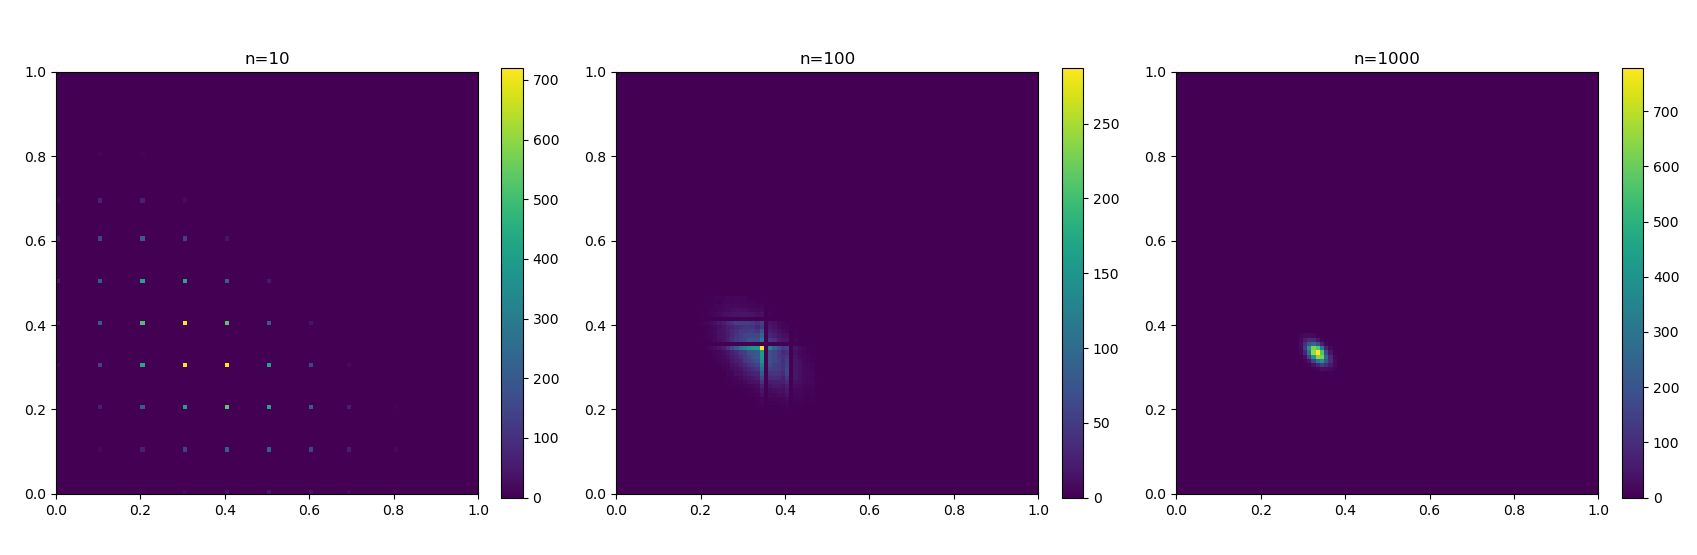
\includegraphics[width=0.8\textwidth]{Images/HW1-hist.png}
		            \end{center}

		      \item {Explain why each histogram in part (h) is an approximate visualization of the pmf $r$, i.e., of the pmf of the random empirical pmf for the given value of $n$.} Explain how the histograms  in part (h) illustrate the law of large numbers. What value is the histogram in part (h) accumulating around for large $n$?

		            \color{blue}
		            In part (c), we showed that $\hat p \approx h$ for large $n$. This gives numerical evidence for the law of large numbers: as $n$ increases, $(\hat p_1, \hat p_2) \to (\frac{1}{3}, \frac{1}{3}) = (h_1, h_2)$. And in fact, this also explains why the historgrams visualize $r$: $r_q$ is the PMF of the empirical PMF of $h$. The histograms show the concentrations of randomly sampled empirical distributions of samples from $h$. Hence, as $\hat p \to h$, with large probability, $r_q \to h$.
		            \color{black}

	      \end{enumerate}



	      \pagebreak

	      %%%%%%%%%%%%%% Indicator Trick %%%%%%%%%%%%%%%%%
	\item{\bf The indicator trick.} Given a domain ${\mathcal D}$ and a subset $A \subseteq \mathcal{D}$, the indicator function, $\ind_A:\mathcal{D}\to \{0,1\}$, is the function that indicates whether or not $x\in\mathcal{D}$ is in $A$:
	      \[
		      \ind_A(x) \triangleq
		      \begin{cases}
			      1 & \text{if $x\in A$}     \\
			      0 & \text{if $x\not\in A$}
		      \end{cases}
	      \]
	      $\ind_A(x)$ is often (maybe even typically) written as $\ind_{x\in A}$.
	      \begin{enumerate}[(a)]
		      \item Let $X$ be a random variable taking values in $\mathcal{D}$ with probability distribution $\Prob$, so $\Prob(A) = \Prob(X\in A)$. Fix $A\in\mathcal{D}$ and let $p = \Prob(A)$. Notice that $\ind_{X \in A}$, being a function of $X$, is itself a random variable. Compute $\Exp[\ind_{X \in A}]$ in terms of $p$.

		            \color{blue}
		            \[\E [\ind_{X \in A}] = 1 \cdot \P(X \in A) + 0 \cdot \P(X \not\in A) = \P(X \in A) = \boxed{p}\]
		            \color{black}

		      \item Using the same $X$, $A$, and $p$, compute $\Var[\ind_{X \in A}]$ (the variance of the random variable $\ind_{X\in A}$).
		            \color{blue}
		            \[\Var[\ind_{X \in A}] = \E[(\ind_{X \in A})^2] - \E[\ind_{X \in A}]^2 = 1^2 \cdot p + 0^2 \cdot (1 - p) - p^2 = \boxed{p - p^2}\]

		            \color{black}

		      \item Suppose that I have $n$ different letters addressed to $n$ different individuals, each living at a different address. I print $n$ envelopes with the correct addresses, but absent-mindedly place the letters randomly into the envelopes. Each envelope gets exactly one letter. Assuming that every placement of letters into envelopes is equally likely, compute the expected number of letters that go to the right individuals. (Hint: for each $k\in\{1,2,\ldots,n\}$ define $Y_k$ to indicate the event that the $k$'th letter goes to the correct address.)

		            \color{blue}
		            Take letters $X_1, \dots, X_n$ on envelopes $\{1, \dots, n\}$ so that $Y_k = \ind\{X_k = k\}$ corresponds to the event that the $k$-th letter ends up in the correct (i.e. $k$-th) envelope.

		            Then, $X$, the number of letters that end up in the correct envelopes, is given by $X = \sum_{k=1}^n Y_k$. By linearity of expectation, we have
		            \[\E[X] = \E\left[\sum_{k=1}^n Y_k\right] = \sum_{k=1}^n \E[Y_k] = \sum_{k=1}^n \E[\ind\{X_k = k\}] = \sum_{k=1}^{n} \P(X_k = k) = \sum_{k=1}^{n} \frac{1}{n} = \boxed{1}\]
		            \color{black}


	      \end{enumerate}

	      Once you set up (c) correctly, it's quite easy to make the calculation. To appreciate the "indicator trick", think about making the same calculation more directly: first compute the probability, say $p_k$, that exactly $k$ letters end up in the correct envelopes, for each $k=1,2,\ldots,n$. Then get the expected value by computing the sum $\sum_{k=1:n} kp_k$.




	      \pagebreak
	      %%%%%%%%%%%%%%%%%% Asymptotics of the multinomial coefficients, heuristically %%%%%%%%%%%%%%%

	\item \tbf{On the asymptotics of $C(\hat{p})$, heuristically.}
	      Most of the discussion of the Gibbs thought experiment was more of an outline than a rigorous derivation.  The key insight was the surprising role of entropy
	      in approximating the number of ways to produce an ensemble with a given empirical empirical distribution, $\hat{p}$.  With the help of the Stirling approximation, we concluded that
	      \begin{equation}
		      \label{eqn:entropy_approx}
		      C(\hat{p}) \approx e^{nH(\hat{p})}
	      \end{equation}
	      where
	      \[
		      C(\hat{p}) \doteq \frac{n!}{(n\hat{p}_1)! \cdots (n\hat{p}_s)!} = \binom{n}{n\hat{p}_1,\dotsc,n\hat{p}_s}
		      \qquad\text{(``the multinomial coefficient")}
	      \]

	      and $H(\hat{p})=-\sum_{x=1:s} \hat{p}_x \log \hat{p}_x$ is Shannon's entropy.

	      The Stirling approximation uses $k^ke^{-k}\sqrt{2\pi k}$ to approximate $k!$, with bounds
	      \begin{equation}
		      \label{eqn:Stirling}
		      e^{\frac{1}{12k +1}} \leq \frac{k!}{k^k e^{-k}\sqrt{2\pi k}}
		      \leq e^{\frac{1}{12k}} \qquad \text{for all $k\geq 1$}
	      \end{equation}

	      If we write $\SSS(k)$ for $k^ke^{-k}\sqrt{2\pi k}$ and define $\SSS(0) = 1$, then $\SSS(k)$ is exact when $k=0$ (since $0! = 1$), and $\SSS(k)$ is an excellent bound in the sense of
	      (\ref{eqn:Stirling}) for all other $k$.  For convenience, we further extend the definition of $\SSS$ by declaring that $\SSS$ evaluated on {\em any} expression means replacing every factorial $k!$ in the expression by $\SSS(k)$, and in particular
	      \[
		      \SSS(C(\hat{p})) =
		      \frac{n^n e^{-n} \sqrt{2\pi n}}
		      {\prod_{x=1}^s n_x^{n_x} e^{-n_x} \sqrt{2\pi n_x}}
	      \]
	      where $n_x \triangleq n\hat{p}_x = \#\{k:X_k=x\}$.

	      The purpose of this problem is to give some justification for the following step that was taken in class (without explanation) while deriving (\ref{eqn:entropy_approx}):
	      for fixed $s$ and empirical probability $\hat{p}$,
	      \[
		      \log\frac{C(\hat{p})}{\SSS(C(\hat{p}))} = O(\frac{1}{n})
	      \]

	      To this end, let ${\cal I} = \{x\in\{1,2,\ldots,s\}\big | \hat{p}_x \neq 0\}$ and show that
	      \[
		      \left| \log\frac{C(\hat{p})}{\SSS(C(\hat{p}))} \right| \leq \frac{1}{12n}\left( 1 + \sum_{x\in {\cal I}}\frac{1}{\hat{p}_x} \right)
	      \]

	      \color{blue}
	      \[ \frac{C(\hat p)}{S(C(\hat p))}
		      = \frac{n!}{\prod_{x \in \mathcal{I}} (n\hat p_x)!}\cdot \frac{\prod_{x \in \mathcal{I}} (n\hat p_x)^{n\hat p_x} e^{n\hat p_x} \sqrt{2\pi n \hat p_x}}{n^n e^{-n} \sqrt{2\pi n}}
		      = \frac{n!}{S(n)} \frac{\prod_{x \in \mathcal{I}} S(n\hat p_x)}{\prod_{x \in \mathcal{I}}  (n \hat p_x)! }
		      = \frac{n!}{S(n)} \prod_{x \in \mathcal{I}} \frac{S(n\hat p_x)}{(n \hat p_x)!} \]

	      \begin{align*}
		      \abs{\log \frac{C(\hat p)}{S(C(\hat p))}} & = \abs{\log \frac{n!}{S(n)} + \sum_{x \in \mathcal{I}} \log \frac{S(n\hat p_x)}{(n \hat p_x)!}}                                                   \\
		                                                & \leq \abs{\log \frac{n!}{S(n)} } + \sum_{x \in \mathcal{I}} \abs{\log \frac{S(n\hat p_x)}{(n \hat p_x)!}} &  & (\text{triangle inequality})       \\
		                                                & \leq \frac{1}{12n} + \sum_{x \in \mathcal{I}} \frac{1}{12n \hat p_x + 1}                                  &  & (\text{by Stirling approximation}) \\
		                                                & \leq \frac{1}{12n} + \sum_{x \in \mathcal{I}} \frac{1}{12n \hat p_x}                                                                              \\
		                                                & = \frac{1}{12n} \left(1 + \sum_{x \in \mathcal{I}} \frac{1}{\hat p_x}\right) \qed
	      \end{align*}
	      \color{black}

	      \pagebreak

	\item {\bf Refresher: working with Gaussian random variables (GRVs).} Given a continuous RV $X$ with probability density function $f$, we will write $X\sim {\cal N}(\mu,\sigma^2)$ (alternatively $f \sim {\cal N}(\mu,\sigma^2)$ to indicate that $X$ has a Gaussian (aka normal) distribution with mean $\mu$ and variance $\sigma^2$):
	      \[
		      f(x) = \frac{1}{\sqrt{2\pi \sigma^2}}e^{-\frac{(x-\mu)^2}{2\sigma^2}}
	      \]
	      \begin{enumerate}[(a)]
		      \item {\bf Sums of independent GRVs.}
		            Linear combinations of {\em independent} Gaussian random variables are Gaussian. Formally, if $X_k\sim{\cal N}(\mu_k,\sigma_k^2)$, for $k=1,\ldots,n$, are $n$ independent Gaussian RVs, and if $a_l \in\R$, for $l=0,1,\ldots,n$, are $n+1$ constants, then $X \triangleq a_0 + \sum_{k=1}^n a_k X_k$ is also Gaussian. Give explicit formulas for the mean ($\mu$) and variance ($\sigma^2$) of $X$ in terms of the $a_k$'s, $\mu_k$'s, and $\sigma_k$'s.

		            \color{blue}
		            Since $X$ is a Gaussian, $\E[X] = \mu$.  Hence,
		            \begin{align*}
			            \mu & = \E[x] = \E\left[a_0 + \sum_{k=1}^{n} a_k X_k\right]         \\
			                & = a_0 + \sum_{k=1}^{n} a_k \E[X_k]  \qquad (\text{linearity}) \\
			                & = a_0 + \sum_{k=1}^{n} a_k \mu_k
		            \end{align*}

		            Further, $\Var[X] = \sigma^2$. Hence,
		            \begin{align*}
			            \sigma^2 & = \Var[X] = \Var\left[a_0 + \sum_{k=1}^{n} a_k X_k\right]                         \\
			                     & = \Var\left[\sum_{k=1}^{n} a_k X_k\right]                                         \\
			                     & = \sum_{i, j}^n a_i a_j \text{cov}(X_i, X_j)                                      \\
			                     & = \sum_{k=1}^n a_k^2 \Var[X_k] \qquad (\text{since } X_i \text{ are independent}) \\
			                     & = \sum_{k=1}^n a_k^2 \sigma_k^2
		            \end{align*}
		            \color{black}


		      \item {\bf Complete the square.}
		            Assume that $X$ is a continuous RV with pdf
		            \[
			            f(x) = c e^{-\frac{1}{4}x^2 + \frac{1}{2}x} \qquad x\in\R
		            \]
		            Show that $X \sim {\cal N}(\mu,\sigma^2)$, and give explicit values for $\mu$, $\sigma^2$, and the normalizing constant $c$. (Hint: complete the square.)

		            \color{blue}
		            With PDF,
		            \begin{align*}
			            f(x) & = c e^{-\frac{1}{4}x^2 + \frac{1}{2}x}           \\
			                 & = c e^{-\frac{1}{4}(x^2 - 2x + 1) + \frac{1}{4}} \\
			                 & = ce^{1/4} \cdot e^{-\frac{(x - 1)^2}{4}}
		            \end{align*}
		            we have that $X \sim {\cal N}(\mu, \sigma^2)$ for $\boxed{c = \frac{e^{-1/4}}{\sqrt{4\pi}}, \mu = 1, \sigma^2 = 2}$.
		            \color{black}

		      \item {\bf A neat trick.} Follow these steps to show that
		            \[
			            \frac{1}{\sqrt{2\pi \sigma^2}} \int_{x=-\infty}^\infty e^{-\frac{(x-\mu)^2}{2\sigma^2}} dx = 1
		            \]
		            for all $\mu$ and $\sigma^2>0$:
		            \begin{enumerate}[i.]
			            \item Use a change of variables to conclude that it would be sufficient to show
			                  \begin{equation}
				                  \label{eqn:1D}
				                  \int_{x=-\infty}^\infty e^{-\frac{x^2}{2}} dx =\sqrt{2\pi}
			                  \end{equation}

			                  \color{blue}
			                  Let $u = \frac{x - \mu}{\sigma}$. Then it suffices to show
			                  \begin{gather*}
				                  \frac{1}{\sigma} \int_{-\infty}^\infty e^{-\frac{(x-\mu)^2}{2\sigma^2}} dx  = \sqrt{2\pi} \\
				                  \frac{1}{\sigma}\int_{-\infty}^\infty e^{-\frac{u^2}{2}} \sigma du = \sqrt{2\pi} \\
				                  \int_{-\infty}^\infty e^{-\frac{u^2}{2}} du = \sqrt{2\pi}
			                  \end{gather*}
			                  \color{black}

			            \item Argue that, instead of showing (\ref{eqn:1D}), it would be sufficient to show
			                  \begin{equation}
				                  \label{eqn:2D}
				                  \int_{x=-\infty}^\infty  \int_{y=-\infty}^\infty e^{-\frac{x^2+y^2}{2}} dxdy =2\pi
			                  \end{equation}

			                  \color{blue}
			                  Let $I = \int_{-\infty}^\infty e^{-\frac{x^2}{2}} dx$. Since it suffices to show $I = \sqrt{2\pi}$, we may write
			                  \begin{align*}
				                  I^2 & = \left(\int_{-\infty}^\infty e^{-\frac{x^2}{2}} dx\right)\left(\int_{-\infty}^\infty e^{-\frac{y^2}{2}} dy\right) \\
				                      & = \int_{-\infty}^\infty  \int_{-\infty}^\infty e^{-\frac{x^2+y^2}{2}} \;dx\,dy = 2\pi
			                  \end{align*}
			                  \color{black}

			            \item Change the double integral in (\ref{eqn:2D}) to polar coordinates and then integrate the left-hand side to get $2\pi$.

			                  \color{blue}
			                  Let $x^2 + y^2 = r^2$, hence
			                  \begin{align*}
				                  I^2 & = \int_{-\infty}^\infty  \int_{-\infty}^\infty e^{-\frac{x^2+y^2}{2}} \;dx\,dy \\
				                      & = \int_{0}^{2\pi} \int_{0}^{\infty} re^{-\frac{r^2}{2}} \;dr\,d\theta          \\
				                      & = \int_0^{2\pi} \left[-e^{-\frac{r^2}{2}}\right]_0^{\infty} \; d\theta         \\
				                      & = \int_0^{2\pi} 1 \; d\theta = 2\pi \qed
			                  \end{align*}
			                  \color{black}

		            \end{enumerate}

	      \end{enumerate}



	      \pagebreak

	\item {\bf Large deviation, continuous random variables.}
	      \label{prob:LD_continuous}
	      Consider $X_{1:n} \triangleq (X_1,\dotsc,X_n)$ drawn $iid$ from the standard normal pdf (prbabilitiy density function)
	      ${\mathcal N}(0,1)$, and let $\sigma_n$ be the standard deviation of the sample mean,
	      $\bar{X}=\frac{1}{n}\sum_{i=1}^n X_i$. The goal is to use experiments to make an informed conjecture about the
	      limit as $n\to\infty$ of the empirical distribution $\hat{p}(X_{1:n})$, given that $\bar{X}$ turns out to be, quite unexpectedly, more than 3.8 standard deviations bigger than its
	      mean, i.e. $\bar{X} > 3.8\sigma_n$. Specifically, with $n$=10,000:
	      \begin{enumerate}[(a)]
		      \item Calculate $\sigma_{10,000}$\footnote{
			            Handy things to remember when computing variances of sums of independent random variables:
			            \begin{enumerate}[(i)]
				            \item If $X$ and $Y$ are independent and $\alpha$ and $\beta$ are scalars, and if $W = \alpha X + \beta Y$, then $\sigma_W^2 = \alpha^2 \sigma_X^2 + \beta^2\sigma_Y^2$
				            \item For any random variable $X$ with mean $\mu_X = \Exp[X]$, $\sigma_X^2 = \Exp[(X-\mu_X)^2] = \Exp[X^2] - \mu_X^2$
			            \end{enumerate}
		            } and the exact probability of the unexpected event: $\P(\bar{X}>3.8\sigma_n)$. Exact means without using the central limit theorem or any Monte Carlo experimentation (though you will need a computer, or at least an old-fashioned lookup table).

		            \color{blue}
		            \begin{align*}
			            \E[\bar X_{10000}]   & = \E\left[\frac{1}{10000}\sum_{i=1}^{10000} X_i\right] = \frac{1}{10000}\sum_{i=1}^{10000} \E[X_i] = 0 \\
			            \Var[\bar X_{10000}] & = \Var\left[\frac{1}{10000}\sum_{i=1}^{10000} X_i\right]                                               \\
			                                 & = \frac{1}{10000^2}\sum_{i=1}^{10000} \Var[X_i] = \frac{1}{10000}
		            \end{align*}

		            Hence,
		            \[\sigma_{10000} = \sqrt{\frac{1}{10000}} = \frac{1}{100}\]
		            and
		            \begin{align*}
			            \P(\bar X > 3.8\sigma_{10000}) & = \P(\bar X > 0.038)                                                                         \\
			                                           & = 1 - \P(\bar X \leq 0.038)                                                                  \\
			                                           & = 1 - \P\left(\frac{\bar X - 0}{\sigma_{10000}} \leq \frac{0.038 - 0}{\sigma_{10000}}\right) \\
			                                           & = 1 - \P(Z \leq 0.38)                                                                        \\
			                                           & = 1 - 0.99993                                                                                \\
			                                           & = \boxed{0.00007}
		            \end{align*}

		            \color{black}

		      \item One way to sample from the conditional distribution on $X_{1:n}$
		            (given that $\bar{X} >3.8\sigma_n$) is to make repeated, independent, draws of all 10,000
		            $iid\ {\mathcal N}(0,1)$ random variables. About how many draws would you expect to need before getting a sample with
		            $\bar{X}>3.8\sigma_{10,000}$?

		            \color{blue}
		            Since $\P(\bar X > 3.8\sigma_{10000}) = 0.00007$, we would expect to need $\frac{1}{0.00007} \approx 14286$ draws before getting a sample with $\bar{X} > 3.8\sigma_{10000}$.
		            \color{black}

		      \item {\color{blue} (Do not submit)} Perform the experiment described in (b). Once you have a sample,
		            display the normalized histogram, and compute the sample mean, the sample standard deviation, and the sample kurtosis.
		            %	Here are some helpful Matlab commands: for a vector ``sample'' (with, say, 10,000 components), you can use 
		            %	\begin{lstlisting}
		            %	histogram(sample,'Normalization','probability')
		            %	disp(['mean: ',num2str(mean(sample))])
		            %	disp(['standard deviation',num2str(std(sample))])
		            %	disp(['kurtosis: ',num2str(kurtosis(sample))])
		            %	\end{lstlisting}

		            \begin{center}
			            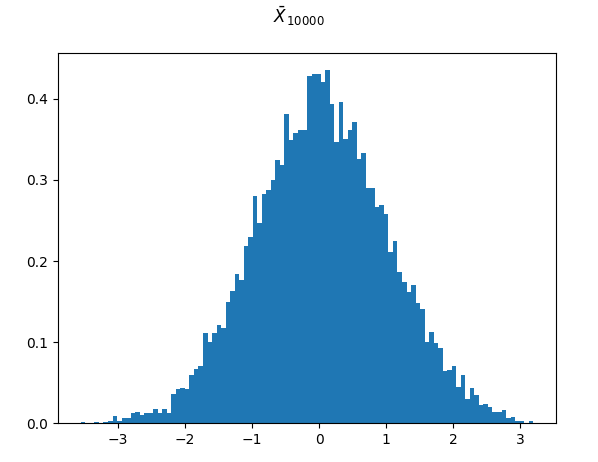
\includegraphics[width=0.6\textwidth]{Images/HW1-normal.png}
		            \end{center}

		            \color{blue}
		            After 8941 draws, we obtained a sample with:
		            \begin{itemize}
			            \item Mean: 0.04337
			            \item Standard deviation: 0.9919
			            \item Kurtosis: -0.0791
		            \end{itemize}
		            \color{black}

		      \item
		            Let $h(x)$ be the standard normal density function, and define
		            the set $B$ by
		            \[
			            B = \big\{g: g\ \text{is a pdf on $\R$ }, E_g[X]>3.8\sigma_{10,000} \big\}1
		            \]
		            and define the density function $f(x)$ by
		            \begin{equation}
			            \label{eqn:LDP}
			            f = \argmin_{g \in B} D(g||h)
		            \end{equation}
		            where $h$ is the standard normal density function and
		            \[
			            D(g||h) = \int_{-\infty}^{\infty} g(x)\log \big(\frac{g(x)}{h(x)}\big) dx
		            \]
		            Use your observations from (c) to make a conjecture about the solution to (\ref{eqn:LDP}). (You can check your answer if you can solve problem \ref{prob:calc_variations}.)

		            \color{blue}
		            Since the histogram in (c) looks like a normal curve, we would expect the solution to (\ref{eqn:LDP}) to look like $q \sim \mathcal{N}(0.38, 1)$
		            \color{black}
	      \end{enumerate}

	      \medskip

	      \hrule

	      \medskip

	      \pagebreak

	\item[] \hspace{-3ex} {\bf For 2610 or for extra credit:}


	      \noindent These problems create careful bounds for some of the approximations used in class.

	\item {\tbf{Rigorous bounds on ${C(\hat{p})}$}.}
	      Fix a positive integer $n$. Let $p=p_{1:s}$ be a pmf with the property that $np$ is a vector of integers, and let $H(p)$ denote the entropy of $p$ computed using $\log_e$ (i.e. $H(p) = -\sum_{i=1}^s p_i \log_e p_i$).
	      \begin{enumerate}
		      \item Prove that there are at most $(n+1)^s$ possible choices of $p$ (i.e., pmfs with the property that $np$ is a vector of integers.)

		            \color{blue}
		            Let $n_i = np_i \in \Z$.

		            Notice
		            \[\sum_{i=1}^{s} p_i = 1 \implies \sum_{i=1}^s n_i = n\]

		            Further, since $p$ is a PMF, $0 \leq p_i \leq 1 \implies 0 \leq n_i \leq n \quad \forall i$.

		            This tells us that
		            \[\left\{n_i \in \Z: 0 \leq n_i \leq n, \sum_{i=1}^s n_i = n\right\} \sub \left\{n_i \in \Z: 0 \leq n_i \leq n\right\} = \{0, 1, 2, \dots, n\}\]

		            Ignoring the constraint $\sum_{i=1}^s n_i = n$ for now, we see that there are $(n+1)^s$ possible choices of $p$ (by assigning a random integer in $[0, n]$ to each of the $s$ elements of $p$).

		            Including the the constraint $\sum_{i=1}^s n_i = n$, we see that there will in fact be many fewer than $(n+1)^s$ possible choices of $p$.
		            \color{black}

		      \item  Prove that
		            \[ \binom{n}{np_1,\dotsc,np_s} \leq e^{nH(p)}  . \]
		            Hint: Let $X_{1:n}$ be iid $p$ and express $\Prob(\widehat p(X_{1:n})=p)$ in terms of $H(p)$ and the multinomial coefficient (and then note that probabilities are always $\leq 1$).

		            \color{blue}
		            Recall
		            \begin{align*}
			            \P(\hat p = p)      & = \binom{n}{np_1 \cdots np_s} \prod_{x=1}^s p_x^{np_x}          \\
			            \log \P(\hat p = p) & = \log \binom{n}{np_1 \cdots np_s} + \sum_{x=1}^s np_x \log p_x \\
			                                & = \log \binom{n}{np_1 \cdots np_s} - n H(p)
		            \end{align*}

		            But then
		            \[\P(\hat p = p) = e^{-nH(p)} \binom{n}{np_1 \cdots np_s} \implies e^{nH(p)} \P(\hat p = p) = \binom{n}{np_1 \cdots np_s}\]

		            However, $\P(\hat p = p) \leq 1$, so
		            \[e^{nH(p)} \geq \binom{n}{np_1 \cdots np_s}\]

		            \color{black}

		      \item Prove that
		            \[  \frac{1}{(n+1)^s} e^{nH(p)} \leq \binom{n}{np_1,\dotsc,np_s} . \]
		            Hint: Let $X_{1:n}$ be iid $p$, and prove that $\Prob(\widehat p(X_{1:n})=p) \geq \Prob(\widehat p(X_{1:n})=q)$ for all valid pmfs $q$. Use this to immediately obtain $1=\sum_q \Prob(\widehat p(X_{1:n})=q) \leq \sum_q \Prob(\widehat p(X_{1:n})=p)$, and then use part (a). You may find this bound useful:
		            For any two positive integers, $a$ and $b$,
		            $a!/b!\geq b^{a-b}$.

		            \color{blue}
		            As before,
		            \begin{align*}
			            \P(\hat p = p) & = \binom{n}{np_1 \cdots np_s} \prod_{x=1}^s p_x^{np_x} = n!\prod_{x=1}^s \frac{p_x^{np_x}}{(np_x)!} \\
			            \P(\hat p = q) & = \binom{n}{nq_1 \cdots nq_s} \prod_{x=1}^s p_x^{nq_x}= n!\prod_{x=1}^s \frac{p_x^{nq_x}}{(nq_x)!}
		            \end{align*}

		            Then, consider
		            \[\frac{\P(\hat p = p)}{\P(\hat p = q)} = \prod_{x=1}^s \frac{p_x^{np_x}}{(np_x)!} \cdot \frac{(nq_x)!}{p_x^{nq_x}} \geq \prod_{x=1}^s p_x^{np_x - nq_x} (np_x)^{nq_x - np_x}  = \prod_{x=1}^s n^{nq_x - np_x}\]

		            Taking the log,
		            \begin{align*}
			            \log \frac{\P(\hat p = p)}{\P(\hat p = q)} & \geq \sum_{x=1}^s (nq_x - np_x) \log n                \\
			                                                       & = n\log n \sum_{x=1}^s (q_x - p_x) = 0                \\
			                                                       & \implies \frac{\P(\hat p = p)}{\P(\hat p = q)} \geq 1 \\
			                                                       & \implies \P(\hat p = p) \geq \P(\hat p = q)
		            \end{align*}

		            In particular, this means that
		            \[1 = \sum_q \P(\hat p = q) \leq \sum_q \P(\hat p = p)\]

		            But from (a),
		            \[1  \leq \sum_q \P(\hat p = p) = \sum_q \binom{n}{np_1 \cdots np_s} \prod_{x=1}^s p_x^{np_x} = (n+1)^s \binom{n}{np_1 \cdots np_s} \prod_{x=1}^s p_x^{np_x}\]
		            \begin{align*}
			            \frac{e^{nH(p)}}{(n+1)^s} & \leq \binom{n}{np_1 \cdots np_s} e^{nH(p)}\prod_{x=1}^s p_x^{np_x}                                 \\
			                                      & = \binom{n}{np_1 \cdots np_s} \exp\left(-\sum_{x=1}^s np_x \log p_x\right)\prod_{x=1}^s p_x^{np_x}
		            \end{align*}

		            \begin{gather*}
			            \log \frac{e^{nH(p)}}{(n+1)^s} \leq \log \binom{n}{np_1 \cdots np_s} - \sum_{x=1}^s np_x \log p_x + \sum_{x=1}^s np_x \log p_x    \\
			            \log \frac{e^{nH(p)}}{(n+1)^s} \leq \log \binom{n}{np_1 \cdots np_s}                                                              \\
			            \frac{e^{nH(p)}}{(n+1)^s}     \leq  \binom{n}{np_1 \cdots np_s} \qed
		            \end{gather*}
		            \color{black}

	      \end{enumerate}

	      \pagebreak

	\item {\bf Relative entropy and likelihood bounds on the empirical distribution.}
	      Let $X_{1:n}$ be iid $h=h_{1:s}$, let $q=q_{1:s}$ be a pmf with the property that $nq$ is a vector of integers, and let
	      \[
		      D(q\|h) \doteq \sum_{i=1}^s q_i \log_e \frac{q_i}{h_i}
	      \]
	      denote relative entropy computed using $\log_e$.
	      %\begin{enumerate}
	      %\item 
	      Use the previous problem to prove that
	      \[ \frac{1}{(n+1)^s} e^{-nD(q\|h)} \leq \Prob(\widehat p(X_{1:n}) = q) \leq e^{-nD(q\|h)} . \]

	      \color{blue}
	      Since
	      \[\P(\hat p = q)  = \binom{n}{nq_1 \cdots nq_s} \prod_{x=1}^s h_x^{nq_x} \]
	      by 9.b,
	      \[\frac{1}{(n+1)^s} e^{nH(q)} \prod_{x=1}^s h_x^{nq_x} \leq \P(\hat p =q) \leq e^{nH(q)} \prod_{x=1}^s h_x^{nq_x} \]
	      so it suffices to show that
	      \[e^{-nD(q \| h)} = e^{nH(q)} \prod_{x=1}^s h_x^{nq_x}\]

	      By definition,
	      \begin{align*}
		      e^{-nD(q\| h)} & = \exp(-n\sum_{i=1}^s q_i \log \frac{q_i}{h_i})         \\
		                     & = \exp(\sum_{i=1}^s -nq_i \log q_i + nq_i \log h_i)     \\
		                     & = e^{nH(q)} \exp\left(\sum_{i=1}^s nq_i \log h_i\right) \\
		                     & = e^{nH(q)} \prod_{x=1}^s h_x^{nq_x}
	      \end{align*}
	      so indeed,
	      \[ \frac{1}{(n+1)^s} e^{-nD(q\|h)} \leq \Prob(\widehat p(X_{1:n}) = q) \leq e^{-nD(q\|h)} \qed\]


	      \color{black}

	      \pagebreak


	\item{\bf Calculus of variations, with constraints.}
	      \label{prob:calc_variations}
	      Consider again the set up in problem (\ref{prob:LD_continuous}).
	      Find a closed-form solution to the optimization problem defined in equation (\ref{eqn:LDP}).
	      Here's an outline, in case you're not familiar with the calculus of variations: (i) introduce Lagrange multipliers, which will be multiplying integrals instead of sums; (ii) replace every instance of $g(x)$ by $g(x)+\epsilon\eta(x)$, where $\eta(x)$ is an arbitrary function;
	      (iii) evaluate the derivative, with respect to $\epsilon$, of the resulting expression at $\epsilon=0$; (iv) use the fact that $\eta$ is arbitrary.

	      \color{red}
	      We want to find a closed form solution to
	      \[f = \argmin_{g \in B} D(g \| h)\]
	      where
	      \begin{itemize}
		      \item $B = \{g: g \text{ pdf on } \R,\; \E_g[X] > 3.8\sigma_{10,000}\}$
		      \item $h$ is the standard normal density function, i.e. $h(x) = \frac{1}{\sqrt{2\pi}}e^{-\frac{x^2}{2}}$
		      \item $D(g \| h) = \int_{-\infty}^{\infty} g(x) \log \frac{g(x)}{h(x)}\; dx$
	      \end{itemize}

	      By definition of $B$, we have constraints
	      \begin{itemize}
		      \item $\int_{-\infty}^{\infty} g(x)\; dx = 1$
		      \item $\int_{-\infty}^{\infty} xg(x)\; dx > 3.8\sigma_{10,000}$
	      \end{itemize}

	      Hence, we seek $g$ which maximizes
	      \[D(g \| h) + \gamma \int_{-\infty}^{\infty} g(x)\; dx + \lambda \int_{-\infty}^{\infty} xg(x)\; dx\]

	      Taking derivatives WRT $g$ and setting to zero, we have
	      \begin{align*}
		      \frac{\partial}{\partial g(x)} & \left[D(g \| h) + \gamma \int_{-\infty}^{\infty} g(x)\; dx + \lambda \int_{-\infty}^{\infty} xg(x)\; dx\right]                                                                                 \\
		                                     & = \frac{\partial}{\partial g(x)} \left[\int_{-\infty}^{\infty} g(x) \log \frac{g(x)}{h(x)}\; dx + \gamma \int_{-\infty}^{\infty} g(x)\; dx + \lambda \int_{-\infty}^{\infty} xg(x)\; dx\right] \\
		                                     & = \frac{\partial}{\partial g(x)} \left[\int_{-\infty}^{\infty} g(x)\left(\log \frac{g(x)}{h(x)} + \gamma + \lambda x\right) \right]
	      \end{align*}
	      \color{black}



	      \pagebreak

	\item {\bf Proof of the LDP.}\footnote{This is a really hard problem, even though you will be guided through it step by step. If you can work through every step, then great. But even if you cannot, it will be well worth your time to give it a try. And of course there will be plenty of opportunities for partial credit.} Let ${\cal S} \triangleq \{q\in[0,1]^s : \sum_x q_x = 1\}$ be the $s$-dimensional probability simplex, i.e., the set of all probability mass functions (pmfs) over the sample space $\{1,\dotsc,s\}$.
	      For any two pmfs $\alpha,\beta \in {\cal S}$, define $\|\alpha - \beta \| = \max_{x=1:s} |\alpha_x - \beta_x |$.
	      Fix $h\in {\cal S}$, let $X_1,X_2,\dotsc$ be iid random variables with common pmf $h$, and define $\widehat p = \widehat p(X_{1:n})$ to be the empirical distribution.  Suppose $B\subseteq{\cal S}$ and define
	      \[ D(B\|h) \triangleq \inf_{q\in B} D(q\|h) . \]
	      (Previous problems are useful throughout this problem.)
	      \begin{enumerate}

		      \item Prove that \[ \limsup_{n\to\infty} \frac{1}{n} \log \Prob(\widehat p(X_{1:n}) \in B) \leq -D(B\|h) . \]

		            \color{blue}
		            Since $B$ is finite, our results above hold and we have
		            \begin{align*}
			            \P(\hat p \in B) & = \sum_{q \in B} \P(\hat p = q)                        \\
			                             & \leq e^{-D(q \| h)}             & \text{by problem 10}
		            \end{align*}
		            so
		            \[\frac{1}{n} \log \P(\hat p \in B) = -D(q \| h)\]

		            Then since $\lim_{n \to \infty} \frac{1}{n} \log \P(\hat p \in B) = 0$,
		            \[\limsup f = \liminf f = \lim f\]
		            we have
		            \begin{align*}
			            \liminf_{n\to\infty} \frac{1}{n} \log \P(\hat p \in B) & \leq\liminf_{n\to \infty} -D(q\|h) \\
			            \limsup_{n\to\infty} \frac{1}{n} \log \P(\hat p \in B) & \leq \inf_{q \in B} -D(q\|h)       \\
		            \end{align*}
		            \color{black}


		      \item Suppose $B$ is an open set\footnote{This means that $B$ is open relative to the topology on ${\cal S}$. $B$ cannot be open in $\mathbb{R}^s$ since it is a subset of ${\cal S}$. To avoid confusion, we might say that $B$ is relatively open in ${\cal S}$, meaning that $B={\cal S}\cap O$ for some open set $O\subseteq\mathbb{R}^s$.} and $h_i > 0$ for all $i=1,\dotsc,s$. Prove that there exists a sequence $q^1,q^2,\dotsc$ of pmfs in $B$ (using superscripts for indices, not powers) with the properties that $D(q^n\|h)\to D(B\|h)$ as $n\to\infty$ and that $\Prob(\widehat p(X_{1:n})=q_n) > 0$ for all $n$ sufficiently large.

		            \color{red}
		            Let $q^* = \arg\inf_{q \in B} D(B \| h)$.

		            Suppose $q^* \in B$. But then since $B$ is open, $\exists q^{\dagger} \in B_{\ep}(q^*)$ such that $D(q^{\dagger} \| h) \leq D(q^* \| h)$, which contradicts that $q^*$ is a lower bound. Hence, $q^* \notin B$.

		            Similarly, suppose $q \notin B$ and $q \notin \Omega$, the boundary of $B$. Then, again, there exists $q^{\dagger} \in B_{\ep}(q)$ such that
		            \[D(q^* \| h) \leq D(q^{\dagger}) \leq D(q \| h) \quad \forall q\in B\]
		            which contradicts that $q^*$ is the greatest lower bound.

		            Hence, $q^* \in \Omega \implies q^* \in \bar B$ since $\bar B = B \cup \Omega$ is the smallest closed set containing $B$. By an equivalent definition of the closure, $\bar B = B \cup X$ where $X$ is the set of limit points of $B$.

		            Since $q^* \notin B$, $q^* \in X$ so $q^*$ is a limit of point of $B$. Hence, there exists a sequence $q^n \in B$ such that $q^n \to q^*$ as $n \to \infty$.

		            Then, by definition of $q^*$, $q^n \to q^* \implies D(q^n \| h) \to D(q^* \| h) = D(B \| h)$ as $n \to \infty$.

		            Finally, to show $\P(\hat p = q_n) > 0$, it suffices to show $q_n \in \Q^s$ for all $n$.
		            \color{black}


		      \item Prove that \[ \liminf_{n\to\infty} \frac{1}{n} \log \Prob(\widehat p(X_{1:n}) \in B) \geq \liminf_{n\to\infty} \frac{1}{n} \log \Prob(\widehat p(X_{1:n}) = q_n) = -D(B\|h)  \]

		      \item[] (Combining (a) and (c) gives \[ \lim_{n\to\infty}   \frac{1}{n} \log \Prob(\widehat p(X_{1:n}) \in B) = -D(B\|h) , \label{e:D} \] which is the first part of the LDP.)

		      \item Prove that
		            \[ \lim_{n\to\infty} \Prob\big(D(\widehat p(X_{1:n})\|h) < D(B\|h)+\delta \ \big| \ \widehat p(X_{1:n}) \in B\big)  = 1  \]
		            for all $\delta > 0$.

		      \item Assume that $p^*\triangleq \argmin_{q\in \overline B} D(q\|h)$ is unique. Show that $D(p^*\|h)=D(B\|h)$ and that
		            \[ \lim_{n\to\infty} \Prob\big( \|\widehat p(X_{1:n})-p^*\|  < \epsilon \ \big| \ \widehat p(X_{1:n})\in B\big) = 1 \]
		            for every $\epsilon > 0$. This is the second part of the LDP.  (Hint: Begin by showing that for each $\epsilon > 0$, there is a $\delta > 0$ such that the event in part (d) is a subset of the event in part (e).)


	      \end{enumerate}
	      \label{last-item}
\end{enumerate}

\end{document}